\paragraph{Task delegation.} Observation requests (a standing person to be detected, recognised or identified) are
delegated to a heterogeneous fleet: half the drones carry a zoom camera and half a fixed wide lens, and their states of
charge range from 12\% to 90\%, as between sorties. Every candidate quotes a request against the shared models: the
energy of the flight out at a corridor-safe altitude, a 60\,s observation and the flight home under the field wind,
and the perception level reached from the best of eight viewpoints around the target, with line of sight and slant
optical depth. Figure~\ref{fig:delegation} compares three awards on the same requests. Awarding the nearest drone, as
a distance-only dispatcher does, completes 42.2\% of requests. Of all its awards (one per request), 34.1\% break the launch reserve, among them
16.2\% that would strand the drone, and 35.8\% send a drone beyond the wind rating (the two overlap in strong wind); and a wide-lens drone is often nearest when a zoom
is needed. A contract net whose perception quote ignores line of sight and the atmosphere never breaks the reserve but
completes only 47.3\%, because it picks drones that cannot resolve the target. The contract net on the shared models
completes 58.6\% of requests, 94.2\% in clear air, never breaks the reserve, and declines the 37.8\% that no drone can
serve safely, mostly in thunderstorms, blizzards and sandstorms. The price is a 10\% longer time to the target (106\,s
against 96\,s), because the best drone is not always the nearest.

\begin{figure}[t]
\centering
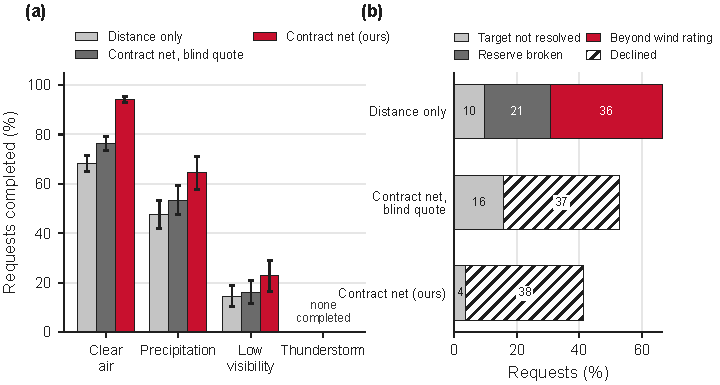
\includegraphics[width=\textwidth]{figures/pdf/delegation.pdf}
\caption{Capability-based delegation, 7 cities, 12 presets, 5 seeds, 30 requests each (12,600 requests per policy).
(a) Requests completed per weather group. (b) Why requests fail: the awarded drone cannot resolve the target, the
flight breaks the launch reserve, the route exceeds the wind rating, or the request is declined because no drone can
serve it}
\label{fig:delegation}
\end{figure}
